\documentclass[aspectratio=169,11pt,t]{beamer}

% ============================================================
% Theme and typography
% ============================================================

\usetheme{Madrid}
\usecolortheme{default}
\usefonttheme{professionalfonts}

\setbeamertemplate{navigation symbols}{}
\setbeamertemplate{headline}{}

\setbeamertemplate{footline}{%
  \leavevmode\hbox{%
  \begin{beamercolorbox}[wd=.82\paperwidth,ht=2.5ex,dp=1.0ex,leftskip=.8em]{author in head/foot}
    CSCI 2406 --- Computer Organization \& Architecture
  \end{beamercolorbox}%
  \begin{beamercolorbox}[wd=.18\paperwidth,ht=2.5ex,dp=1.0ex,rightskip=.8em]{date in head/foot}
    \hfill\insertframenumber/\inserttotalframenumber
  \end{beamercolorbox}}
}

\setbeamersize{
  text margin left=0.65cm,
  text margin right=0.65cm
}

\setbeamerfont{frametitle}{size=\Large, series=\bfseries}
\setbeamerfont{block title}{size=\normalsize, series=\bfseries}
\setbeamertemplate{blocks}[rounded][shadow=false]

% Block vertical padding adjustments
\addtobeamertemplate{block begin}{\vspace{0.1em}}{\vspace{0.1em}}
\addtobeamertemplate{block end}{}{\vspace{0.2em}}

% Base list item separation
\setbeamertemplate{itemize/enumerate body begin}{\setlength{\itemsep}{4pt}}
\setbeamertemplate{itemize/enumerate subbody begin}{\setlength{\itemsep}{2pt}}

% ============================================================
% Packages
% ============================================================

\usepackage[T1]{fontenc}
\usepackage{lmodern}
\usepackage{iftex}
\ifPDFTeX
  \usepackage[scale=0.92]{sourcecodepro}
\else
  \usepackage{fontspec}
  \setmonofont[Scale=0.92]{Source Code Pro}
\fi
\usepackage{amsmath}
\usepackage{booktabs}
\usepackage{array}
\usepackage{colortbl}
\usepackage{tikz}

\usetikzlibrary{
  arrows.meta,
  positioning,
  shapes.geometric,
  calc,
  decorations.pathreplacing
}

% ============================================================
% Colors
% ============================================================

\definecolor{navy}{RGB}{24,43,68}
\definecolor{deepblue}{RGB}{45,88,130}
\definecolor{lightblue}{RGB}{235,242,250}
\definecolor{softgray}{RGB}{245,247,250}
\definecolor{darkgray}{RGB}{25,28,32}
\definecolor{gold}{RGB}{200,145,35}

\setbeamercolor{palette primary}{bg=navy,fg=white}
\setbeamercolor{palette secondary}{bg=deepblue,fg=white}
\setbeamercolor{frametitle}{bg=navy,fg=white}
\setbeamercolor{title}{fg=white}
\setbeamercolor{subtitle}{fg=white}
\setbeamercolor{author}{fg=white}
\setbeamercolor{date}{fg=white}
\setbeamercolor{titlelike}{fg=white}
\setbeamercolor{block title}{bg=deepblue,fg=white}
\setbeamercolor{block body}{bg=lightblue,fg=darkgray}
\setbeamercolor{normal text}{fg=darkgray,bg=white}

% ============================================================
% Formatting shortcuts
% ============================================================

\setlength{\parskip}{0pt}

\newcommand{\key}[1]{\textbf{#1}}
\newcommand{\bits}[1]{\texttt{#1}}
\newcommand{\hex}[1]{\texttt{0x#1}}
\newcommand{\code}[1]{\texttt{#1}}
% Simple fixed-width bit-field box for instruction diagrams.
% Coordinates use bit positions; set x scale in the tikzpicture.
\newcommand{\bfld}[5]{%
  \pgfmathsetmacro{\cx}{#1 + #3/2}%
  \fill[#5] (#1,#2) rectangle ++(#3,0.72);%
  \draw[navy,line width=0.7pt] (#1,#2) rectangle ++(#3,0.72);%
  \node[font=\scriptsize\ttfamily,text height=1.5ex,text depth=0.35ex,align=center,text=darkgray] at (\cx,#2+0.36) {#4};%
}
\newcommand{\bitnote}[3]{%
  \node[font=\tiny,text height=1.5ex,text depth=0.35ex,align=center,text=darkgray] at (#1,#2) {#3};%
}
\newcommand{\codeblock}[1]{%
  \begingroup\small\ttfamily\setlength{\fboxsep}{5pt}\colorbox{softgray}{\begin{minipage}{0.92\linewidth}#1\end{minipage}}\endgroup%
}


% Section divider macro
\newcommand{\sectiondivider}[2]{%
\begin{frame}[plain]

\begin{tikzpicture}[remember picture,overlay]
\fill[navy] (current page.south west) rectangle (current page.north east);
\fill[gold] (current page.south west)
  rectangle ([yshift=.15cm]current page.south east);
\end{tikzpicture}

\vspace*{\fill}

\begin{minipage}{0.94\textwidth}
\raggedright
\hyphenpenalty=10000
\exhyphenpenalty=10000

{\color{gold}\large\bfseries #1\par}

\vspace{0.3cm}

{\color{white}\fontsize{22}{26}\selectfont\bfseries
#2\par}

\end{minipage}

\vspace*{\fill}

\end{frame}
}

% ============================================================
% Metadata
% ============================================================

\title[Topic 9]{
  Machine Code \& AArch64 Instruction Encoding
}

\subtitle{
  Fixed-width instruction words, encoding fields, data-processing,\\
  memory access, and branch instructions
}

\author{
  Computer Organization \& Architecture
}

\date{}

% ============================================================
% Document
% ============================================================


\begin{document}

% ============================================================
% ============================================================

\begin{frame}[plain]
\begin{tikzpicture}[remember picture,overlay]
\fill[navy] (current page.south west) rectangle (current page.north east);
\fill[gold] (current page.south west) rectangle ([yshift=.15cm]current page.south east);
\end{tikzpicture}

\vspace*{\fill}

\begin{minipage}{0.88\textwidth}
{\color{gold}\normalsize\bfseries
CSCI 2406 \;|\; Computer Organization \& Architecture \;|\; TOPIC 9
\par}

\vspace{0.25cm}

{\color{white}\fontsize{24}{28}\selectfont\bfseries
Machine Code \& AArch64\\[0.08cm]Instruction Encoding
\par}

\vspace{0.35cm}

{\color{white!80}\large
Instruction words, encoding fields, immediates, memory operations,\\and branch targets in AArch64
\par}
\end{minipage}

\vfill

{\color{white!70}\small
Dr. J. Burns
\par}

\vspace*{\fill}
\end{frame}

% ============================================================
% ============================================================

\begin{frame}{Topic 9 Outline}
\setbeamertemplate{enumerate item}{%

\begin{tikzpicture}[baseline=-0.65ex]
\fill[black!20] (0.035,-0.035) circle (0.145);
\fill[blue!35!black] (0,0) circle (0.145);
\fill[blue!55!black] (-0.012,0.012) circle (0.123);
\fill[blue!65!white] (-0.027,0.035) circle (0.096);
\fill[blue!45!black] (0.008,-0.018) circle (0.102);
\node[text=white,font=\scriptsize\sffamily,inner sep=0pt] at (0,0) {\insertenumlabel};
\end{tikzpicture}}
\setbeamercolor{item projected}{fg=white,bg=blue!50!black}
\begin{enumerate}\setlength{\itemsep}{13pt}
\item \key{Machine Code and 32-bit Instruction Words}
\item \key{AArch64 Encoding Families}
\item \key{Data-Processing Encodings}
\item \key{Memory Instruction Encodings}
\item \key{Branch Instruction Encodings}
\end{enumerate}
\end{frame}

% ============================================================
% ============================================================

\sectiondivider{Section 1}{Machine Code and 32-bit Instruction Words}

% ============================================================
% ============================================================

\begin{frame}{From Assembly to Machine Code}

\begin{itemize}\setlength{\itemsep}{6pt}
  \item A processor repeatedly \key{fetches}, \key{decodes}, and \key{executes} instructions.
  \item During fetch--decode--execute, the processor fetches a 32-bit instruction word from memory and interprets its bit fields.
  \item This topic starts with the earlier step: how an AArch64 assembly instruction is encoded as that fixed \key{32-bit} machine instruction.
\end{itemize}

\vspace{0.18cm}

\begin{center}
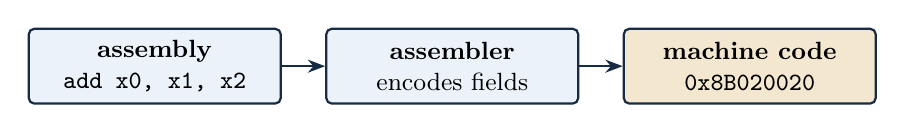
\begin{tikzpicture}[
  font=\small,
  node distance=0.55cm,
  procbox/.style={
    draw=navy,
    line width=0.8pt,
    rounded corners=2pt,
    minimum width=3.2cm,
    minimum height=0.95cm,
    align=center,
    fill=lightblue
  },
  wordboxstyle/.style={
    procbox,
    fill=gold!22
  },
  arr/.style={
    -{Stealth[length=2.2mm]},
    draw=navy,
    line width=0.8pt
  }
]

\node[procbox] (asm) {\textbf{assembly}\\\code{add x0, x1, x2}};
\node[procbox, right=of asm] (assembler) {\textbf{assembler}\\encodes fields};
\node[wordboxstyle, right=of assembler] (wordbox) {\textbf{machine code}\\\hex{8B020020}};

\draw[arr] (asm) -- (assembler);
\draw[arr] (assembler) -- (wordbox);

\end{tikzpicture}
\end{center}


\small In memory, \hex{8B020020} is stored as bytes \code{20 00 02 8B} in increasing address order (A64 instruction byte order).
\end{frame}

% ============================================================
% ============================================================

\begin{frame}{AArch64 Encoding Essentials}
\begin{itemize}\setlength{\itemsep}{7pt}
\item Every A64 instruction occupies 32 bits (4 bytes), with operation and operand fields. Consecutive instruction addresses differ by 4 bytes.
\item Different instruction families use different field layouts.
\item Register fields are normally 5 bits, encoding register numbers 0--31.
\item There are 31 general-purpose registers. Register number 31 denotes the zero register or stack pointer, depending on the instruction and operand.
\item Identify the instruction form before interpreting its fields.
\end{itemize}
\end{frame}

% ============================================================
% ============================================================



% ============================================================
% ============================================================

\sectiondivider{Section 2}{AArch64 Encoding Families}

\begin{frame}{Where Do Opcode Patterns Come From?}
\begin{itemize}\setlength{\itemsep}{8pt}
\item \key{Look up the instruction format in Arm's ISA reference.} It specifies the fixed bits and field positions for that instruction form.
\item \key{Select the form first, for example:} \code{add x5, x6, x7} uses a shifted-register form; \code{add x5, x6, \#24} uses an immediate form with a different field layout.
\item \key{Fill the selectors:} width, operation, flag update, shift type, access size, or addressing mode choose among related encodings.
\item \key{Insert the operands:} register numbers, immediates, and offsets occupy the remaining fields.
\item \key{A prefix is not necessarily one opcode field:} leading bits may combine fixed family bits with selectors. Each table states the form and bit positions to which its patterns apply.
\end{itemize}
\end{frame}

\begin{frame}{From Instruction Word to Operand Fields}
\small
\code{Rd}: destination; \code{Rn}/\code{Rm}: source registers (\code{Rn} is the memory base).\\
\code{Rt}: transferred register; \code{immN}: an N-bit immediate; \code{cond}: condition selector.
\begin{center}
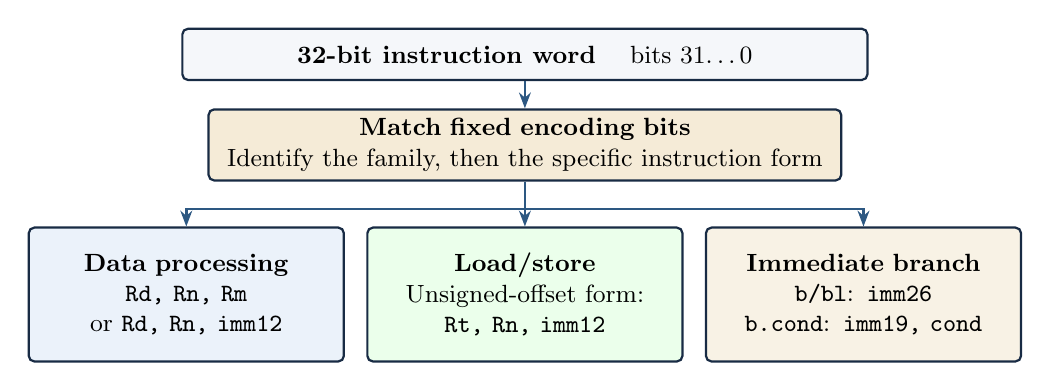
\begin{tikzpicture}[
  font=\small,
  stage/.style={draw=navy,line width=0.8pt,rounded corners=2pt,align=center},
  family/.style={stage,text width=3.65cm,minimum height=1.7cm,inner sep=5pt},
  flow/.style={-{Stealth[length=2mm]},draw=deepblue,line width=0.9pt}
]
\node[stage,fill=softgray,minimum width=8.7cm,minimum height=0.65cm] (word) at (0,0)
  {\textbf{32-bit instruction word} \quad bits 31\ldots0};
\node[stage,fill=gold!18,text width=7.8cm,minimum height=0.85cm] (decode) at (0,-1.15)
  {\textbf{Match fixed encoding bits}\\Identify the family, then the specific instruction form};
\draw[flow] (word) -- (decode);
\node[family,fill=lightblue] (data) at (-4.3,-3.05)
  {\textbf{Data processing}\\\code{Rd, Rn, Rm}\\or \code{Rd, Rn, imm12}};
\node[family,fill=green!8] (mem) at (0,-3.05)
  {\textbf{Load/store}\\Unsigned-offset form:\\ \code{Rt, Rn, imm12}};
\node[family,fill=gold!12] (branch) at (4.3,-3.05)
  {\textbf{Immediate branch}\\\code{b/bl}: \code{imm26}\\\code{b.cond}: \code{imm19, cond}};
\draw[flow] (decode.south) -- ++(0,-0.35) -| (data.north);
\draw[flow] (decode.south) -- (mem.north);
\draw[flow] (decode.south) -- ++(0,-0.35) -| (branch.north);
\end{tikzpicture}
\end{center}
The selected form determines each field\textquotesingle s meaning. The following slides define the layouts and values.
\end{frame}


% ============================================================
% ============================================================



% ============================================================
% ============================================================



% ============================================================
% ============================================================



% ============================================================
% ============================================================



% ============================================================
% ============================================================



% ============================================================
% ============================================================

\sectiondivider{Section 3}{Data-Processing Encodings}

% ============================================================
% ============================================================

\begin{frame}{add/sub: Shifted-Register Form}
\small
Here we compare two versions of \code{add}: one uses the second source register directly; the other shifts its value left before adding.

\begin{center}
\small Sample instructions: \code{add x5, x6, x7}\qquad\code{add x5, x6, x7, lsl \#3}
\end{center}

\vspace{0.1cm}

\begin{center}
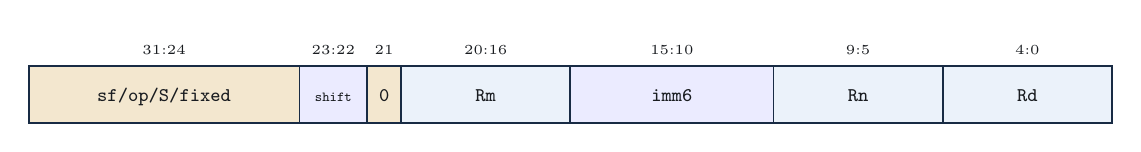
\begin{tikzpicture}[x=0.43cm,y=1cm]
  \bfld{0}{0}{8}{sf/op/S/fixed}{gold!22}
  \bfld{8}{0}{2}{\tiny shift}{blue!8}
  \bfld{10}{0}{1}{0}{gold!22}
  \bfld{11}{0}{5}{Rm}{lightblue}
  \bfld{16}{0}{6}{imm6}{blue!8}
  \bfld{22}{0}{5}{Rn}{lightblue}
  \bfld{27}{0}{5}{Rd}{lightblue}
  \bitnote{4}{0.95}{31:24}
  \bitnote{9}{0.95}{23:22}
  \bitnote{10.5}{0.95}{21}
  \bitnote{13.5}{0.95}{20:16}
  \bitnote{19}{0.95}{15:10}
  \bitnote{24.5}{0.95}{9:5}
  \bitnote{29.5}{0.95}{4:0}
\end{tikzpicture}
\end{center}

\vspace{0.15cm}

\begin{itemize}\setlength{\itemsep}{4pt}
  \item \code{sf/op/S/fixed} will be defined on the next slide.
  \item \code{Rd}: destination; \code{Rn}: first source; \code{Rm}: second source.
  \item Both examples use \code{shift=00} (lsl). The first implies \code{lsl \#0}.
  \item \code{imm6} changes from \code{000000} to \code{000011} for \code{lsl \#3}: the second example computes \code{x5 = x6 + (x7 << 3)}.
  \item Bit 21 is fixed at \code{0} in this arithmetic form.
\end{itemize}

\end{frame}

% ============================================================
% ============================================================

\begin{frame}{Deriving the Prefix: \texttt{add x5, x6, x7}}
\small
Select \key{add/sub (shifted register)}. Bits 31:21 have this structure:
\begin{center}
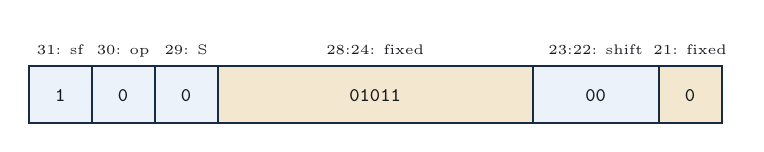
\begin{tikzpicture}[x=0.8cm,y=1cm]
\bfld{0}{0}{1}{1}{lightblue}
\bfld{1}{0}{1}{0}{lightblue}
\bfld{2}{0}{1}{0}{lightblue}
\bfld{3}{0}{5}{01011}{gold!22}
\bfld{8}{0}{2}{00}{lightblue}
\bfld{10}{0}{1}{0}{gold!22}
\bitnote{0.5}{0.95}{31: sf}
\bitnote{1.5}{0.95}{30: op}
\bitnote{2.5}{0.95}{29: S}
\bitnote{5.5}{0.95}{28:24: fixed}
\bitnote{9}{0.95}{23:22: shift}
\bitnote{10.5}{0.95}{21: fixed}
\end{tikzpicture}
\end{center}
\par\renewcommand{\arraystretch}{1.1}
\par\vspace{3pt}{\centering
\begin{tabular}{@{}lll@{}}
\toprule
\textbf{Field} & \textbf{Choice} & \textbf{Reason} \\
\midrule
\code{sf} & \code{1} & 64-bit \code{x} operands; \code{0} selects 32-bit \code{w} operands \\
\code{op} & \code{0} & Add; \code{1} selects subtract \\
\code{S} & \code{0} & Preserve NZCV flags; \code{1} updates them \\
Fixed bits & \code{01011} and \code{0} & Fixed bits for this encoding class \\
\code{shift} & \code{00} & lsl; the absent shift defaults to lsl \code{\#0} \\
\bottomrule
\end{tabular}\par}\vspace{3pt}
\vspace{0.18cm}

\key{Concatenate:} \code{1 | 0 | 0 | 01011 | 00 | 0 = 10001011000}.
The separate \code{imm6} field is \code{000000} for shift amount zero.
\end{frame}


\begin{frame}{Common Arithmetic Register Patterns}
\small
All rows use 64-bit shifted-register forms: \code{sf=1}, \code{shift=00} (lsl), and bit 21 fixed at 0.

\par\vspace{8pt}{\centering
\renewcommand{\arraystretch}{1.25}
\begin{tabular}{@{}lll@{}}
\toprule
\textbf{Instruction} & \textbf{op / S} & \textbf{Prefix 31:21} \\
\midrule
\code{add} & \code{0 / 0} & \code{1|0|0|01011|00|0} \\
\code{adds} & \code{0 / 1} & \code{1|0|1|01011|00|0} \\
\code{sub} & \code{1 / 0} & \code{1|1|0|01011|00|0} \\
\code{subs} & \code{1 / 1} & \code{1|1|1|01011|00|0} \\
\bottomrule
\end{tabular}
\par}
\vspace{0.2cm}
\setbeamertemplate{itemize item}{\color{navy}\raisebox{0.15ex}{\rule{0.65ex}{0.65ex}}}
\begin{itemize}\setlength{\itemsep}{5pt}
\item Prefix field order: \code{sf | op | S | 01011 | shift | 0}.
\item \code{op} selects addition (0) or subtraction (1); \code{S=1} updates NZCV.
\item \code{imm6} selects the shift amount. For 32-bit forms, set \code{sf=0}; shift amounts are 0--31.
\end{itemize}
\end{frame}

\begin{frame}{Encoding Example: \texttt{add x5, x6, x7}}

\begin{columns}[T,onlytextwidth]

\column{0.48\textwidth}
\begin{block}{Register Numbers}
\[
\begin{aligned}
Rd &= x5 = 00101 \\
Rn &= x6 = 00110 \\
Rm &= x7 = 00111
\end{aligned}
\]
\end{block}

\column{0.48\textwidth}
\begin{block}{Operation Fields}
\[
\begin{aligned}
\text{operation} &= \text{add} \\
\text{operand size} &= 64\text{-bit} \\
\text{shift amount} &= 0
\end{aligned}
\]
\end{block}

\end{columns}

\vspace{0.2cm}

\begin{center}
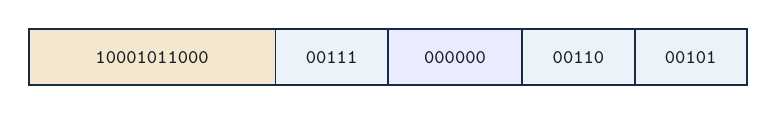
\begin{tikzpicture}[x=0.285cm,y=1cm]
  \bfld{0}{0}{11}{10001011000}{gold!22}
  \bfld{11}{0}{5}{00111}{lightblue}
  \bfld{16}{0}{6}{000000}{blue!8}
  \bfld{22}{0}{5}{00110}{lightblue}
  \bfld{27}{0}{5}{00101}{lightblue}
\end{tikzpicture}
\end{center}

\vspace{0.1cm}

\centering
The prefix comes from \code{sf/op/S/fixed/shift}; now insert the operands:
\[
\bits{10001011000\;00111\;000000\;00110\;00101}
= \hex{8B0700C5}.
\]

\end{frame}

% ============================================================
% ============================================================

\begin{frame}{add/sub: Immediate Form}
Now we move on to the immediate form, where the second operand is a constant encoded in the instruction.

\begin{center}
Sample instruction: \code{add x5, x6, \#24}
\end{center}

\vspace{0.1cm}

\begin{center}
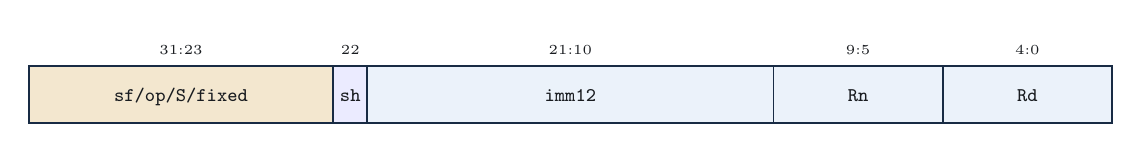
\begin{tikzpicture}[x=0.43cm,y=1cm]
  \bfld{0}{0}{9}{sf/op/S/fixed}{gold!22}
  \bfld{9}{0}{1}{\scriptsize sh}{blue!8}
  \bfld{10}{0}{12}{imm12}{lightblue}
  \bfld{22}{0}{5}{Rn}{lightblue}
  \bfld{27}{0}{5}{Rd}{lightblue}
  \bitnote{4.5}{0.95}{31:23}
  \bitnote{9.5}{0.95}{22}
  \bitnote{16}{0.95}{21:10}
  \bitnote{24.5}{0.95}{9:5}
  \bitnote{29.5}{0.95}{4:0}
\end{tikzpicture}
\end{center}

\vspace{0.15cm}

\begin{itemize}\setlength{\itemsep}{5pt}
  \item The immediate field is 12 bits wide.
  \item Bit 22, \code{sh}: 0 means no shift; 1 means shift the immediate left by 12 bits. Bit 23 is fixed at 0.
  \item This format is common for address arithmetic and small integer constants.
\end{itemize}

\end{frame}

% ============================================================
% ============================================================

\begin{frame}{Common Arithmetic Immediate Patterns}
\small
add/sub (immediate) uses \code{sf | op | S | 100010 | sh | imm12 | Rn | Rd}.
The six fixed bits \code{100010} occupy bits 28:23; \code{sh} is bit 22.
\vspace{0.16cm}
\par\renewcommand{\arraystretch}{1.25}
\par\vspace{3pt}{\centering
\begin{tabular}{@{}llll@{}}
\toprule
\textbf{64-bit form} & \textbf{op} & \textbf{S} & \textbf{Prefix 31:23} \\
\midrule
\code{add Xd, Xn, \#imm}  & \code{0} & \code{0} & \code{1|0|0|100010} \\
\code{adds Xd, Xn, \#imm} & \code{0} & \code{1} & \code{1|0|1|100010} \\
\code{sub Xd, Xn, \#imm}  & \code{1} & \code{0} & \code{1|1|0|100010} \\
\code{subs Xd, Xn, \#imm} & \code{1} & \code{1} & \code{1|1|1|100010} \\
\bottomrule
\end{tabular}\par}\vspace{3pt}
\vspace{0.2cm}
\begin{block}{Derive the add Immediate Prefix}
\code{sf=1, op=0, S=0}: \code{1 | 0 | 0 | 100010 = 100100010}.\\
For \code{\#24}, choose \code{sh=0} and encode 24 directly in \code{imm12}. With \code{sh=1}, the immediate is shifted left by 12 bits.
\end{block}

\end{frame}

\begin{frame}{Encoding Example: \texttt{add x5, x6, \#24}}

\begin{columns}[T,onlytextwidth]
\column{0.48\textwidth}
\begin{block}{Operands}
\[
\begin{aligned}
Rd &= x5 = 00101 \\
Rn &= x6 = 00110 \\
\text{imm12} &= 24 = 000000011000
\end{aligned}
\]
\end{block}

\column{0.48\textwidth}
\begin{block}{Instruction Meaning}
\[
\code{x5 = x6 + 24}
\]
The immediate value is part of the instruction word.
\end{block}
\end{columns}

\vspace{0.2cm}

\begin{center}
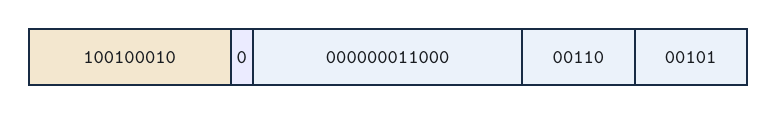
\begin{tikzpicture}[x=0.285cm,y=1cm]
  \bfld{0}{0}{9}{100100010}{gold!22}
  \bfld{9}{0}{1}{0}{blue!8}
  \bfld{10}{0}{12}{000000011000}{lightblue}
  \bfld{22}{0}{5}{00110}{lightblue}
  \bfld{27}{0}{5}{00101}{lightblue}
\end{tikzpicture}
\end{center}

\vspace{0.1cm}

\centering
\code{add x5, x6, \#24} is encoded as \hex{910060C5}.
\par\vspace{0.12cm}\small\raggedright
Immediate rules depend on the instruction form. Constants outside this form may require another instruction form or a sequence of instructions.

\end{frame}

% ============================================================
% ============================================================



% ============================================================
% ============================================================



\begin{frame}{Decoding an Instruction Word}
\small
\key{Given:} \hex{8B020020}. Use the reference patterns, then interpret the fields for that form.
\begin{center}
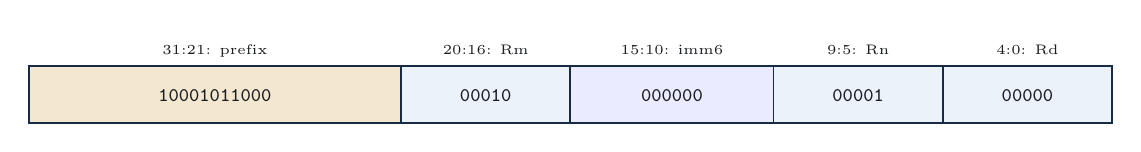
\begin{tikzpicture}[x=0.43cm,y=1cm]
\bfld{0}{0}{11}{10001011000}{gold!22}
\bfld{11}{0}{5}{00010}{lightblue}
\bfld{16}{0}{6}{000000}{blue!8}
\bfld{22}{0}{5}{00001}{lightblue}
\bfld{27}{0}{5}{00000}{lightblue}
\bitnote{5.5}{0.95}{31:21: prefix}
\bitnote{13.5}{0.95}{20:16: Rm}
\bitnote{19}{0.95}{15:10: imm6}
\bitnote{24.5}{0.95}{9:5: Rn}
\bitnote{29.5}{0.95}{4:0: Rd}
\end{tikzpicture}
\end{center}
\begin{enumerate}\setlength{\itemsep}{8pt}
\item \key{Identify the form:} \code{1|0|0|01011|00|0} selects 64-bit \code{add}, without flag updates, using lsl.
\item \key{Read the operands:} \code{Rm=2}, \code{Rn=1}, \code{Rd=0}; \code{imm6=0} means no shift.
\item \key{Reconstruct:} \code{add x0, x1, x2}.
\end{enumerate}
\vspace{0.18cm}
\begin{block}{Decoding Rule}
Identify the form before interpreting the fields. The same bit positions can have different meanings in another form.
\end{block}
\end{frame}

\sectiondivider{Section 4}{Memory Instruction Encodings}

% ============================================================
% ============================================================

\begin{frame}{Scaled Offsets Depend on Access Size}

\small
\setlength{\abovedisplayskip}{4pt}
\setlength{\belowdisplayskip}{4pt}
In unsigned-offset loads/stores, the 12-bit \code{imm12} field stores the \key{byte offset divided by the access size}. The processor multiplies it back:
\[
\text{address} = \text{base} + \text{imm12} \times \text{access size}
\]

\vspace{0.05cm}

\begin{center}
\small
\par\vspace{3pt}{\centering
\begin{tabular}{lll}
\toprule
Instruction kind & Access size & Encoded immediate meaning \\
\midrule
\code{ldrb}/\code{strb} & 1 byte & byte offset \\
\code{ldrh}/\code{strh} & 2 bytes & byte offset divided by 2 \\
\code{ldr w}/\code{str w} & 4 bytes & byte offset divided by 4 \\
\code{ldr x}/\code{str x} & 8 bytes & byte offset divided by 8 \\
\bottomrule
\end{tabular}\par}\vspace{3pt}
\end{center}

\vspace{0.05cm}

\key{For 8-byte accesses:}
\begin{itemize}\setlength{\itemsep}{3pt}
\item \key{Unsigned, scaled \code{imm12}:} 0 to +32,760 bytes, in steps of 8 --- greater forward reach.
\item \key{Signed, unscaled \code{imm9}:} $-256$ to $+255$ bytes, in steps of 1 --- short reach in both directions.
\end{itemize}
\vspace{0.05cm}
Scaling trades finer offset steps for greater reach; signed offsets allow access below the base address.

\end{frame}

\begin{frame}{Load/Store Instruction Encoding}

\begin{center}
Sample instruction: \code{ldr x5, [x6, \#16]}
\end{center}

\vspace{0.1cm}

\begin{center}
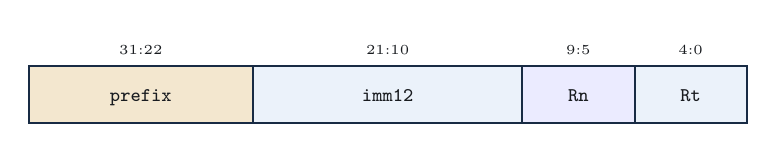
\begin{tikzpicture}[x=0.285cm,y=1cm]
  \bfld{0}{0}{10}{prefix}{gold!22}
  \bfld{10}{0}{12}{imm12}{lightblue}
  \bfld{22}{0}{5}{Rn}{blue!8}
  \bfld{27}{0}{5}{Rt}{lightblue}
  \bitnote{5}{0.95}{31:22}
  \bitnote{16}{0.95}{21:10}
  \bitnote{24.5}{0.95}{9:5}
  \bitnote{29.5}{0.95}{4:0}
\end{tikzpicture}
\end{center}

\vspace{0.1cm}

\begin{itemize}\setlength{\itemsep}{4pt}
  \item \code{Rt} is the register loaded or stored.
  \item \code{Rn} is the base address register.
  \item \code{imm12} stores byte offset / access size in this unsigned-offset form.
  \item For a 64-bit \code{ldr}: \(\text{address} = \code{x6} + 8 \times \text{imm12}\).
\end{itemize}

\end{frame}

% ============================================================
% ============================================================

\begin{frame}{Memory Prefix: Width, Addressing Form and Operation}
\small
Bits 31:22 combine five fields. \code{opc} means operation code; \code{VR} selects the register class (0: general-purpose; 1: SIMD/floating-point).
\par\vspace{7pt}{\centering
\renewcommand{\arraystretch}{1.22}
\begin{tabular}{@{}llll@{}}
\toprule
\textbf{Bits} & \textbf{Field} & \textbf{Choice for \code{ldr x5}} & \textbf{Meaning} \\
\midrule
31:30 & \code{size} & \code{11} & 8-byte access; \code{10} selects 4 bytes \\
29:27 & Fixed & \code{111} & Fixed bits for these load/store forms \\
26 & \code{VR} & \code{0} & General-purpose integer registers \\
25:24 & Form & \code{01} & Unsigned scaled offset, no writeback \\
23:22 & \code{opc} & \code{01} & Load; \code{00} selects store \\
\bottomrule
\end{tabular}\par}\vspace{8pt}
\vspace{0.12cm}
\key{64-bit \code{ldr}:} \code{11 | 111 | 0 | 01 | 01}.\\[0.1cm]
For \code{str}, keep width and addressing form; change \code{opc} from \code{01} to \code{00}.
\end{frame}

\begin{frame}{Common Memory Instruction Patterns}
\small
Use the field order \code{size | fixed | VR | form | opc}. All rows use unsigned-offset addressing \code{[Xn|SP, \#offset]}, with no base update.
\vspace{0.12cm}
\par\renewcommand{\arraystretch}{1.16}
\par\vspace{3pt}{\centering
\begin{tabular}{@{}lllll@{}}
\toprule
\textbf{Transfer} & \textbf{Bytes} & \textbf{size} & \textbf{opc} & \textbf{Prefix 31:22} \\
\midrule
\code{str Wt}  & 4 & \code{10} & \code{00} & \code{10|111|0|01|00} \\
\code{ldr Wt}  & 4 & \code{10} & \code{01} & \code{10|111|0|01|01} \\
\code{str Xt}  & 8 & \code{11} & \code{00} & \code{11|111|0|01|00} \\
\code{ldr Xt}  & 8 & \code{11} & \code{01} & \code{11|111|0|01|01} \\
\bottomrule
\end{tabular}\par}\vspace{3pt}
\vspace{0.15cm}

\key{Complete each word:} \code{prefix | imm12 | Rn | Rt}. The encoded \code{imm12} equals byte offset divided by the number of bytes transferred.
\end{frame}

\begin{frame}{Encoding Example: \texttt{ldr x5, [x6, \#16]}}

\begin{columns}[T,onlytextwidth]
\column{0.48\textwidth}
\begin{block}{Operands}
\[
\begin{aligned}
Rt &= x5 = 00101 \\
Rn &= x6 = 00110 \\
\#16 &= 2 \times 8\text{ bytes}
\end{aligned}
\]
\end{block}

\column{0.48\textwidth}
\begin{block}{Encoded Offset}
\[
\text{imm12} = 2 = 000000000010
\]
The instruction stores the scaled value, not the byte offset directly.
\end{block}
\end{columns}

\vspace{0.2cm}

\begin{center}
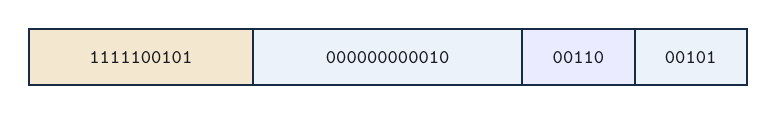
\begin{tikzpicture}[x=0.285cm,y=1cm]
  \bfld{0}{0}{10}{1111100101}{gold!22}
  \bfld{10}{0}{12}{000000000010}{lightblue}
  \bfld{22}{0}{5}{00110}{blue!8}
  \bfld{27}{0}{5}{00101}{lightblue}
\end{tikzpicture}
\end{center}

\vspace{0.1cm}

\centering
\code{ldr x5, [x6, \#16]} is encoded as \hex{F94008C5}.
\par\vspace{0.1cm}\small\raggedright
For \code{str x5, [x6, \#16]}, keep the address fields and change \code{opc} from \code{01} to \code{00}: \hex{F90008C5}. Now \code{Rt} is the source.

\end{frame}

% ============================================================
% ============================================================



% ============================================================
% ============================================================

\begin{frame}{Offset, Pre-Index and Post-Index: What Changes?}
\small
Each example starts separately with \code{x6 = 0x1000}. All three load 8 bytes into \code{x5}. \key{Writeback} means updating the base register, \code{x6}.
\par\vspace{4pt}{\centering
\renewcommand{\arraystretch}{1.2}
\begin{tabular}{@{}llll@{}}
\toprule
\textbf{Instruction} & \textbf{Address read} & \textbf{Final \code{x6}} & \textbf{Offset field} \\
\midrule
\code{ldr x5, [x6, \#16]}  & \code{0x1010} & \code{0x1000} & \code{imm12 = 2} \\
\code{ldr x5, [x6, \#16]!} & \code{0x1010} & \code{0x1010} & \code{imm9 = 16} \\
\code{ldr x5, [x6], \#16}  & \code{0x1000} & \code{0x1010} & \code{imm9 = 16} \\
\bottomrule
\end{tabular}\par}\vspace{4pt}
\begin{itemize}\setlength{\itemsep}{4pt}
\item \key{Offset:} add the offset for the access; leave the base unchanged. The unsigned \code{imm12} is scaled: $16/8=2$.
\item \key{Pre-index:} update the base, then access the updated address.
\item \key{Post-index:} access the old base address, then update the base.
\end{itemize}
\vspace{0.1cm}
Pre/post forms encode a signed \key{byte offset} in \code{imm9}: no division by access size. Their range is $-256$ to $255$ bytes.
\end{frame}

\begin{frame}{Addressing Modes: Encoding Reference}
\small
Reference layout: focus on offset scaling and base updates; exact mode-bit positions need not be memorised.
\begin{center}
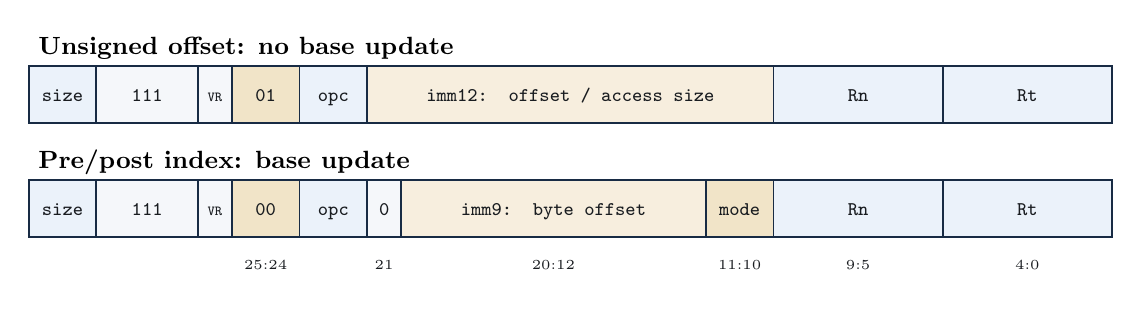
\begin{tikzpicture}[x=0.43cm,y=1cm]
\node[anchor=west,font=\small\bfseries] at (0,2.85) {Unsigned offset: no base update};
\bfld{0}{1.9}{2}{size}{lightblue}
\bfld{2}{1.9}{3}{111}{softgray}
\bfld{5}{1.9}{1}{\tiny VR}{softgray}
\bfld{6}{1.9}{2}{01}{gold!25}
\bfld{8}{1.9}{2}{opc}{lightblue}
\bfld{10}{1.9}{12}{imm12: offset / access size}{gold!15}
\bfld{22}{1.9}{5}{Rn}{lightblue}
\bfld{27}{1.9}{5}{Rt}{lightblue}
\node[anchor=west,font=\small\bfseries] at (0,1.4) {Pre/post index: base update};
\bfld{0}{0.45}{2}{size}{lightblue}
\bfld{2}{0.45}{3}{111}{softgray}
\bfld{5}{0.45}{1}{\tiny VR}{softgray}
\bfld{6}{0.45}{2}{00}{gold!25}
\bfld{8}{0.45}{2}{opc}{lightblue}
\bfld{10}{0.45}{1}{0}{softgray}
\bfld{11}{0.45}{9}{imm9: byte offset}{gold!15}
\bfld{20}{0.45}{2}{mode}{gold!25}
\bfld{22}{0.45}{5}{Rn}{lightblue}
\bfld{27}{0.45}{5}{Rt}{lightblue}
\bitnote{7}{0.12}{25:24}
\bitnote{10.5}{0.12}{21}
\bitnote{15.5}{0.12}{20:12}
\bitnote{21}{0.12}{11:10}
\bitnote{24.5}{0.12}{9:5}
\bitnote{29.5}{0.12}{4:0}
\end{tikzpicture}
\end{center}
\begin{itemize}\setlength{\itemsep}{5pt}
\item \key{Form bits 25:24:} \code{01} for unsigned offset; \code{00} for the pre/post forms shown. Their bit 21 is also fixed at \code{0}.
\item \key{Mode bits 11:10:} \code{11} selects pre-index; \code{01} selects post-index.
\item In unsigned-offset form, bits 11:10 are part of \code{imm12}; there is no separate mode field there.
\end{itemize}
\end{frame}



% ============================================================
% ============================================================



% ============================================================
% ============================================================


% ============================================================
% ============================================================



% ============================================================
% ============================================================

\sectiondivider{Section 5}{Branch Instruction Encodings}

\begin{frame}{Common Immediate Branch Patterns}
\small
The signed displacement counts 4-byte instruction steps: target = branch PC + displacement $\times 4$. PC is the address of the branch itself.
\par\vspace{4pt}
\code{b}/\code{bl} use \code{op | 00101}: \code{op=0} branches; \code{op=1} also saves a return address. Conditional branches use the fixed prefix \code{01010100}, then a displacement and condition field.
\par\vspace{3pt}{\centering
\renewcommand{\arraystretch}{1.1}
\begin{tabular}{@{}llll@{}}
\toprule
\textbf{Instruction} & \textbf{Fixed leading bits} & \textbf{Displacement field} & \textbf{cond (3:0)} \\
\midrule
\code{b label} & \code{0|00101} (31:26) & \code{imm26} (25:0) & --- \\
\code{bl function} & \code{1|00101} (31:26) & \code{imm26} (25:0) & --- \\
\code{b.eq label} & \code{01010100} (31:24) & \code{imm19} (23:5) & \code{0000} \\
\code{b.ne label} & \code{01010100} (31:24) & \code{imm19} (23:5) & \code{0001} \\
\code{b.lt label} & \code{01010100} (31:24) & \code{imm19} (23:5) & \code{1011} \\
\bottomrule
\end{tabular}\par}\vspace{3pt}
\begin{itemize}\setlength{\itemsep}{4pt}

\item \key{Conditional branches:} bit 4 is fixed at \code{0}; \code{cond} selects EQ (Z=1), NE (Z=0), or signed LT (N differs from V).
\item \code{bl} writes the return address, PC + 4, to \code{x30}.
\end{itemize}
\end{frame}



\begin{frame}{Branch Example: Forward Target}
\small
\key{Reference PC = address of the branch itself.} Encoded immediate = (target $-$ PC) / 4.
\vspace{0.12cm}

\begin{columns}[T,onlytextwidth]
\column{0.48\textwidth}
\begin{block}{Code Shape}
\small
\par\vspace{3pt}{\centering
\begin{tabular}{ll}
\code{0x100:} & \code{b target} \\
\code{0x104:} & \code{add x0, x0, \#1} \\
\code{0x108:} & \code{sub x1, x1, \#1} \\
\code{0x10c:} & \code{add x2, x2, \#1} \\
\code{0x110:} & \code{target: sub x3, x3, \#1}
\end{tabular}\par}\vspace{3pt}
\end{block}

\column{0.48\textwidth}
\begin{block}{Offset}
\[
\begin{aligned}
\Delta &= \hex{110} - \hex{100} \\
       &= 16\text{ bytes} \\
\text{imm26} &= 16/4 = 4
\end{aligned}
\]
\end{block}
\end{columns}

\vspace{0.2cm}

\begin{center}
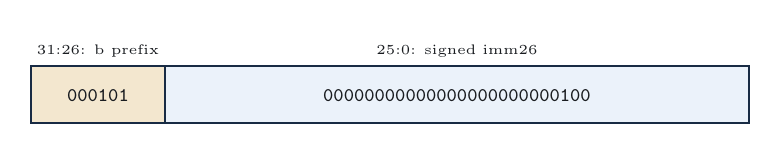
\begin{tikzpicture}[x=0.285cm,y=1cm]
  \bfld{0}{0}{6}{000101}{gold!22}
  \bfld{6}{0}{26}{00000000000000000000000100}{lightblue}
  \bitnote{3}{0.95}{31:26: b prefix}
  \bitnote{19}{0.95}{25:0: signed imm26}
\end{tikzpicture}
\end{center}

\vspace{0.1cm}

\centering
\code{b target}: positive displacement, \code{imm26=4}; word \hex{14000004}.

\end{frame}



% ============================================================
% ============================================================

\begin{frame}{Conditional Branch Example: \texttt{b.eq}}

\small
\code{b.cond} tests NZCV flags: signed \code{imm19} is scaled by 4; bits 3:0 select the condition, and bit 4 is fixed at 0.
\vspace{0.12cm}
\begin{columns}[T,onlytextwidth]
\column{0.48\textwidth}
\begin{block}{Target Offset}
\[
\begin{aligned}
\text{current PC} &= \hex{100} \\
\text{target} &= \hex{110} \\
\text{imm19} &= 4
\end{aligned}
\]
\end{block}

\column{0.48\textwidth}
\begin{block}{Condition Field}
\[
\code{eq} = 0000
\]
The branch is taken when the Z flag is set.
\end{block}
\end{columns}

\vspace{0.2cm}

\begin{center}
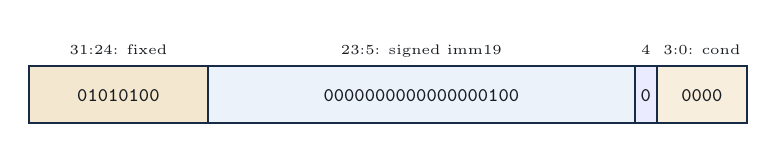
\begin{tikzpicture}[x=0.285cm,y=1cm]
  \bfld{0}{0}{8}{01010100}{gold!22}
  \bfld{8}{0}{19}{0000000000000000100}{lightblue}
  \bfld{27}{0}{1}{0}{blue!8}
  \bfld{28}{0}{4}{0000}{gold!15}
  \bitnote{4}{0.95}{31:24: fixed}
  \bitnote{17.5}{0.95}{23:5: signed imm19}
  \bitnote{27.5}{0.95}{4}
  \bitnote{30}{0.95}{3:0: cond}
\end{tikzpicture}
\end{center}

\vspace{0.1cm}

\centering
\code{b.eq target} is encoded as \hex{54000080}.

\end{frame}

% ============================================================
% ============================================================



% ============================================================
% ============================================================



% ============================================================
% ============================================================



% ============================================================
% ============================================================



% ============================================================
% ============================================================



% ============================================================
% ============================================================

\begin{frame}{Branch Example: Backward Loop}
\small
Assume \code{x0=0} and \code{x1} is a positive iteration count. The branch returns to an earlier instruction while \code{x1} is nonzero.
\vspace{0.12cm}
\begin{columns}[T,onlytextwidth]
\begin{column}{0.54\textwidth}
\begin{block}{Loop Code (Instruction Addresses Shown)}
\ttfamily\small
0x200: loop: add x0, x0, \#1\\[0.08cm]
0x204: \phantom{loop: }subs x1, x1, \#1\\[0.08cm]
0x208: \phantom{loop: }b.ne loop
\end{block}
\end{column}
\begin{column}{0.42\textwidth}
\begin{block}{Signed Displacement}
\[
\begin{aligned}
\text{PC} &= \hex{208} \\
\text{target} &= \hex{200} \\
\Delta &= \hex{200}-\hex{208} = -8 \\
\text{imm19} &= -8/4 = -2
\end{aligned}
\]
\end{block}
\end{column}
\end{columns}
\vspace{0.12cm}
For $-2$: write $+2$ in 19 bits (17 zeros followed by \code{10}), invert all bits, then add 1. This gives \code{1111111111111111110} (\hex{7FFFE}); \code{cond=0001} selects NE.
\begin{center}
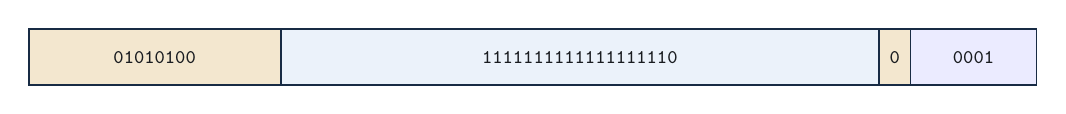
\begin{tikzpicture}[x=0.4cm,y=1cm]
\bfld{0}{0}{8}{01010100}{gold!22}
\bfld{8}{0}{19}{1111111111111111110}{lightblue}
\bfld{27}{0}{1}{0}{gold!22}
\bfld{28}{0}{4}{0001}{blue!8}
\end{tikzpicture}
\end{center}
\key{Check:} \code{0x208 + (-2 * 4) = 0x200}. Instruction word: \hex{54FFFFC1}.\\[0.05cm]
\end{frame}

\begin{frame}{Common Encoding Mistakes}

\begin{itemize}\setlength{\itemsep}{7pt}
  \item Treating a register number as decimal text instead of a binary field.
  \item Forgetting that AArch64 register fields are usually 5 bits.
  \item Encoding a byte offset directly when the immediate field is scaled.
  \item Adding a pipeline offset to PC instead of using the branch instruction address.
  \item Reading little-endian memory bytes as if they were the printed instruction word.
\end{itemize}

\vspace{0.2cm}

\begin{block}{Practical Habit}
Write the bit ranges first, then fill in the fields. Do not try to guess the final hexadecimal word too early.
\end{block}

\end{frame}

% ============================================================
% ============================================================

\begin{frame}{Topic 9: Summary}
\small
\setbeamerfont{itemize/enumerate body}{size=\small}
\begin{itemize}\setlength{\itemsep}{9pt}
\item \key{Instruction words and forms:} A64 instructions occupy 32 bits (4 bytes), stored little-endian. Select the form, look up its fixed pattern, then interpret its fields.
\item \key{Data processing:} \code{op} selects add/subtract and \code{S} controls NZCV updates. Register shifts use \code{shift}/\code{imm6}; arithmetic immediates use \code{imm12}/\code{sh}.
\item \key{Memory:} unsigned offsets are scaled by access size. Pre/post-index forms use signed byte offsets and update the base; the mode determines which address is accessed.
\item \key{PC-relative branches:} target = branch PC + signed immediate $\times 4$. \code{b}/\code{bl} use \code{imm26}; \code{b.cond} uses \code{imm19} and a 4-bit condition. \code{bl} saves PC + 4 in \code{x30}.
\end{itemize}
\end{frame}

% ============================================================
% ============================================================

\begin{frame}{Self-Test Questions: Instruction Words}
\small
Use the reference tables; fixed binary patterns need not be memorised. Show how you choose the variable fields.
\setbeamerfont{itemize/enumerate body}{size=\small}
\begin{enumerate}\setlength{\itemsep}{8pt}
\item How many bytes does an A64 instruction occupy? For \hex{8B020020}, list the four bytes in increasing memory-address order.
\item In the add/sub shifted-register form, what do \code{sf}, \code{op}, and \code{S} select? Which values encode a 64-bit subtraction that updates NZCV?
\item For \code{add x5, x6, x7}, give \code{Rd}, \code{Rn}, and \code{Rm} as 5-bit values. What happens to \code{shift} and \code{imm6} when \code{lsl \#3} is added?
\item For \code{add x5, x6, \#24}, give \code{imm12} and \code{sh}. What would setting \code{sh=1} do to the immediate value?
\item Split \code{10001011000} into its fixed and selector fields. Which selector bits change for \code{subs x5, x6, x7}?
\end{enumerate}
\end{frame}

% ============================================================
% ============================================================

\begin{frame}{Self-Test Questions: Memory and Branches}
\small
\setbeamerfont{itemize/enumerate body}{size=\small}
\begin{enumerate}\setlength{\itemsep}{8pt}
\item In \code{ldr x5, [x6, \#16]}, why is \code{imm12=2}? Which field identifies the base register?
\item For an 8-byte access, compare the offset range and step size of unsigned scaled \code{imm12} and signed unscaled \code{imm9}. Which can address below the base?
\item Each time starting with \code{x6=0x1000}, compare the address read and final \code{x6} for offset, pre-index and post-index \code{ldr} with \code{\#16}. Explain when the base register changes.
\item Compare \code{ldr x5, [x6, \#16]} with \code{str x5, [x6, \#16]}. What is the role of \code{x5} in each, and does either update \code{x6}?
\item A \code{b} at \hex{100} targets \hex{110}; a \code{b.ne} at \hex{208} targets \hex{200}. Calculate each signed immediate and give its field width. Which PC is the reference, and where is NE encoded?
\end{enumerate}
\end{frame}

% ============================================================
% ============================================================



% Encoding references: Arm A64 ISA instruction descriptions, add (shifted register),
% add (immediate), ldr/str/ldrb/strb/ldrh/strh
% (immediate). Official collection:
% https://documentation-service.arm.com/static/67e40f3398aa3c3b6eea6a85
% Arm instruction descriptions, HTML presentation:
% https://www.scs.stanford.edu/~zyedidia/arm64/index.html
\end{document}